
\newtheorem{defn}{Definition} 


\section{Generation of Proof Obligations for Java Bytecode}\label{verifCond}
Once source specification gets compiled in a suitable form, we are ready to perform a procedure for establishing code correctness.
We propose a definition and an implementation of a Weakest Precondition Calculus (WPC) for Java bytecode.
Taking as input the compiled JML specification we are able to generate proof obligations for properties expressed in JML.
Checking partial or total correctness of a class is done by checking partial or total correctness of the bytecode of every method in the class with respect to its specification.

WPC has firstly been defined by Dijkstra (~\cite{WPCDS},~\cite{DisDij}) for imperative structured languages over the language control structures. However bytecode programs lack structure thus WPC for bytecode is carried over the execution graph determined by the bytecode. The algorithm that is proposed here involves three steps:  construction of the execution graph, its transformation to an acyclic one and finally application the WPC over it. The transformation of the execution graph into an acyclic graph is necessary in order to make the calculus terminate. The WPC is defined for method calls and abrupt exceptional termination. In our model we treat instance fields as overriding functions in rather the same way as in \cite{ProBor}. WPC is defined as a predicate transformer over bytecode instructions, named \texttt{wp} with the following signature: 
\begin{center} \texttt{wp} : \texttt{STMT} $\longrightarrow$ \texttt{Predicate} $\longrightarrow$ \texttt{Predicate}\end{center}

The rest of this chapter will discuss the definition of \texttt{wp}, and the code analysis and abstractions necessary to perform the calculus.
%\subsection{Weakest Precondition Calculus}\label{wp}
%Weakest precondition function is a predicate transformer function that for a given statement \texttt{stmt} and a predicate $\psi$ returns the weakest precondition that should be established in the prestate of \texttt{stmt} such that $\psi$ holds after statement's execution (see~\cite{DisDij}). Formally the signature of the function is :
%\begin{center} \texttt{wp} : \texttt{STMT} $\longrightarrow$ \texttt{Predicate} $\longrightarrow$ \texttt{Predicate}\end{center}
%Bytecode programs are considered as a set of execution paths. Correctness of a program implies that all execution paths are correct and vice versa. Thus we are verifying that every execution path is correct.
%\subsection{Well formed bytecode programs}\label{wf}
First programs are assumed to respect some reasonable constraints: hereafter we define what we consider as a well formed bytecode program.
\begin{defn}[Well formed bytecode programs] A bytecode program is well formed if and only if:
\begin{itemize}
\item it has exactly one entry point,
\item for every loop there is exactly one entry point,
\item inner loops must terminate execution before the loop in which they are declared.
\item No recursive subroutines.  Every path in a subroutine must end with a \texttt{ret} or a \texttt{return} instruction. 

%Only \texttt{jsr} instructions may jump to a subroutine. The instructions of subroutine are disjoint from the rest of the bytecode. No instruction belonging to a subroutine may jump outside the subroutine code. Every execution path in a subroutine terminates with a \texttt{ret} instruction. For every execution path \texttt{ret n} must jump exactly to the instruction that follows the corresponding \texttt{jsr} instruction. %No two subroutines may end with the same \texttt{ret}.
\end{itemize}
\label{wf}
\end{defn}
The last point of the constraint list is verified by the Java bytecode verifier as specified in \cite{VMSpec}, chapter 4.8.2. We assume that the code passing through our verification procedure is verified by the Java bytecode verifier.
Also it should be pointed out that standard Java compilers produce a code that respects all the requirements stated above.
%The idea is that once the verification condition for a path is done it is discharged and a theorem prover will try to prove it. In this way theorem prover will deal with smaller formulas.
%A well formed program is considered correct only iff every execution path of the program is correct. An execution path is correct iff its verification condition is provable.%Thus if the proof fails for some execution path the verification condition generator can be switched off in this way avoiding unnecessary calculations.

In order to verify  bytecode program correctness the execution graph is transformed into an acyclic graph, by eliminating some edges. Informally these edges connect the end and the start of a loop.
The first step of this process is the definition of the notion of block, a block will correspond to a node in the execution graph.
%As we treat instructions that are loop ends in a special way, in the rest of the chapter we will use the name \texttt{loop\_end} instruction.


\subsection{Execution graph}
We denote by $\Gamma  = ( \Omega, \ll)$ the execution graph of a
bytecode $\Pi$ where the set of nodes $\Omega$ is the set of
blocks. The set of edges $\ll$ defines the execution relation
between blocks.Using standard terminology \cite{ARUCom1986}, a
basic block is a code segment that has no unconditional jump or
conditional branch statements except for possibly the last
statement, and none of its statements, except possibly the first,
is a target of any jump or branch statement. The formal definition of block follows
below.
%\begin{defn}[A block]
% \label{blockDef}
% is a list of bytecode instructions $\tt{[i_{j}, i_{j+1} ... i_{j + n}]} $ $\tt{n \ge 0 }$ such that:
%\begin{enumerate}
%\item the last instruction $\tt{i_{j + n}}$  is a \texttt{jump},
%\texttt{return}, \texttt{ret}, \texttt{jsr}, \texttt{athrow}
%instruction, or an instruction that is followed by an instruction
% \item the first instruction $\tt{i_{j}}$ is either the entry point instruction of
%the code or a jump target, or an instruction following a
%\texttt{jump} instruction. 
%
%\item the rest of the instructions are sequential instructions, i.e. no one of the following types of
%instruction: \texttt{jump}, \texttt{return}, \texttt{ret},
%\texttt{jsr} instruction, a target of a \texttt{jump}, neither an
%instruction that is followed by an instruction that is a target of
%a \texttt{jump} instruction.
%\end{enumerate}
%\end{defn}

We denote a block that starts at instruction $\tt{i_{j}}$
respectively by \blockm{j}. Let's have the bytecode $\Pi$ and the
set of its blocks  be $\wp$. The edges ( $\ll \ \subseteq \wp \ \times \ \wp $ ) define the order of block execution.

\begin{defn}[Execution relation between blocks]\label{execRel}
\begin{tabbing}
\\Let \=  have \= the block \blockm{j} such that  it ends with instruction $\tt{i_{k}}$ and \\
it is not a return instruction\\
\>  if $\tt{i_{k}}$ = \texttt{if\_cond n} then   \blockm{j} $\ll$ \blockm{n} and \blockm{j}  $\ll $ \blockm{k+1}  \\
\>  if $\tt{i_{k}}$ = \texttt{goto n} then \blockm{j} $\ll$ \blockm{n} \\
\>  if $\tt{i_{k}}$ = \texttt{jsr n} then \blockm{j} $\ll$ \blockm{n} \\
\>  if $\tt{i_{k}}$ = \texttt{athrow} then \blockm{j} $\ll$ \blockm{n} for all \texttt{n}, such that \blockm{n} is the first\\
\> \> block of an exception handler that protects $\tt{i_{k}}$ \\
\>  if  $\tt{i_{k}}$ = \texttt{ret n} then  \blockm{j} $\ll$ \blockm{s}\\
\> \> for all s that are indexes of instruction following \\
\> \> a \texttt{jsr} to the subroutine that ends with $\tt{i_{k}}$ instruction\\
\>  else \blockm{j} $ \ll  $ \blockm{k+1}
\end{tabbing}
\end{defn}
%We say that $\tt{instr_{i}} $ is a precedent of $\tt{instr_{j}}$  and that  $\tt{instr_{j}}$ is next to  $\tt{instr_{i}}$ if $\tt{instr_{i}} \ll \tt{instr_{j}} $ , the same for blocks that are in the same relation.
We say that there exists a path between \blockm{i} and \blockm{j} and we note it with  \pathm{i}{j}, if there exists blocks \blockm{s_{1}}... \blockm{s_{n}} such that \blockm{i}$\ll$ \blockm{s_{1}}$\ll$ \blockm{s_{2}}... \blockm{s_{n}}$\ll$ \blockm{j}
\begin{defn}[Loop Definition]
\label{defLoop}
Let's have a well formed program $\Pi$. We say that \blockm{s} is the start block of loop $l$ in $\Pi$ and \blockm{e} is the end block of $l$ if:
\begin{itemize}
\item there exists a path in the execution graph starting at the entry block \blockm{entry} (i.e. the one that starts with the entry instruction) of $\Pi$ and that passes first through \blockm{s} and later through \blockm{e}, i.e.\blockm{entry} $\ll^{*}$ \blockm{s} $\ll^{*}$ \blockm{e}
\item \blockm{e} $\ll$ \blockm{s}
\end{itemize}
\end{defn}

%Loops are represented as cycles in the execution graph. Every loop has a unique name $ \tt{ loop_{i}}$  Every loop $\tt{loop_{i}}$ in a well formed program is defined uniquely by two  instructions - the first instruction of the loop  $\tt{loop^{i}_{start}}$  and the last instruction of the loop $\tt{loop^{i}_{end}}$  and by definition they are in relation $\ll$.

%Relation $\ll$ defines also an execution relation between blocks $\ll$ (we use the same name for the instruction and block execution relation)
%\begin{defn}{Execution relation between blocks}
%\label{execRel}
%Let $\tt{b^{1}}$ and $\tt{b^{2}}$ are blocks. $\tt{b^{1}} \ll \tt{b^{2}} \iff \tt{b^{1}_{end}} \ll \tt{b^{2}_{start}}$.
%\end{defn}


\subsection{Acyclic Execution Graph} \label{graph}
We consider the acyclic graph $\Gamma^1 = ( \Omega, \ll^1)$ obtained from the execution graph $\Gamma  = ( \Omega, \ll)$ of a well formed bytecode $ \Pi $. The set of nodes $\Omega$ is the set of  blocks in the program and the relation  $\ll^1 $ is a subset of the  execution relation $\ll$.
\begin{defn}[Acyclic Execution relation]
\label{acyclicExRel}
Let's have the well formed bytecode program $\Pi$ and let have in $\Pi$ the two blocks  \blockm{i} and   \blockm{j}. We say that \blockm{i} $\ll^{1}$ \blockm{j} iff
\begin{itemize}
\item \blockm{i} $\ll$ \blockm{j}
\item and block \blockm{i} and block \blockm{j} are not the end and the start blocks respectively of the same loop, see loop definition~\ref{defLoop}.
\end{itemize}
\end{defn}

%Naturally $\ll^1$ defines a relation between blocks for which we use the same notation $\ll^1$ .
Both the cyclic and acyclic graphs of the bytecode of method \texttt{half} at Fig.~\ref{halfBC} is at Fig. ~\ref{blockBC}. Blocks are represented by boxes. Black arrows stand for relation $\ll^1$. Dashed arrows represent relation $\ll$.

\begin{figure}[p]
\begin{center}
\begin{tabular}{rl}
 0 & iconst\_0\\ 
 1 & istore\_2\\
 2 & iload\_1\\
 3 & istore\_3\\%[-2mm]
 4 & goto 13 (+9)\\%[-2mm]
 7 & iinc 2 by 1\\%[-2mm]
10 & iinc 1 by 254\\%[-2mm]
13 & iload\_1\\%[-2mm]
14 & iconst\_1\\%[-2mm]
15 & if\_icmpgt 7 (-8)\\%[-2mm]
18 & iload\_2\\%[-2mm]
19 & ireturn\\%[-2mm]
\end{tabular}
\end{center}
\caption{the bytecode of method \texttt{half}}
\label{halfBC}
\end{figure}

\begin{figure}[p]
\begin{center}
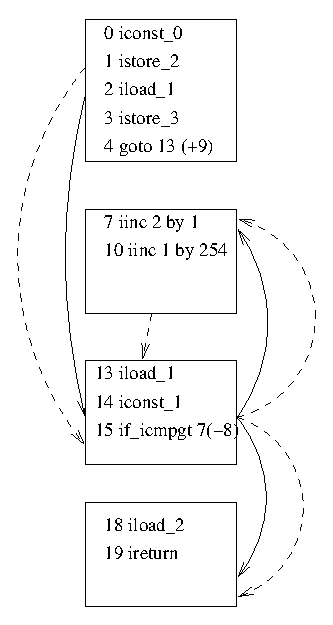
\epsfig{file=graph.eps}
\end{center}
\caption{bytecode blocks of bytecode at Figure ~\ref{halfBC}}
\label{blockBC}
\end{figure}

Now a path in $\Gamma^1$  is a list of blocks between which is established a relation $\ll^1$ and that starts at the entry point instruction and whose last block is a block that does not have next block.

% A path ending with a block that is an end of a loop must establish in its poststate the invariant of the corresponding loop. A path ending with a return must respect the posctondition specified for the bytecode.

%Paths ending with an \texttt{athrow} are treated in a particular way. In general it is not always possible to determine statically the dynamic type of the exception thrown. We determine the most specific type of the exception thrown by an overloading function. Once it is determined it is either an exception type that is handled, i.e. then the weakest precondition will be calculated upon the weakest precondition of the exception handler, or it is not a caught exception in which case the proof obligation will be calculated upon the declared exceptional postcondition.

\subsection{Bytecode Weakest Precondition}
We can now define a weakest precondition on an acyclic execution graph. This is done in three steps: WPC on an execution path, WPC on a block of an execution path, WPC on a bytecode instruction of a block.
\paragraph{WPC for an Execution Path: }
Under the assumption that a bytecode respects the conditions stated in definition~\ref{wf}, we construct the abstract execution graph $\Gamma^1$ as stated in~\ref{graph}. A backwards tracing is done for every execution path in $\Gamma^1$ . The algorithm is:
\begin{enumerate}
\item Calculate for the leaves of the execution tree their weakest preconditions
    \begin{itemize}
    \item for all the leaves of the execution tree that terminate with a \texttt{return} instruction it will calculate its weakest precondition upon the postcondition declared in the specification attribute of the method where the block appears
    \item for all the leaves of the execution tree that terminate with an \texttt{athrow} instruction the exception type will be approximated by an overriding function during the calculus. Thus its weakest precondition will be calculated either upon the weakest precondition of the exception handler of the approximated type if the exception is caught or upon the exceptional postcondition for the approximated exception type that is thrown.
    \item for every block b that terminates with an instruction that is the end of some loop in the bytecode  it will calculate its weakest precondition upon the loop invariant specified.
    \end{itemize}

\item the calculated weakest precondition of a block b is the postcondition  for any block b' such that b' $\ll^1$ b. Calculate upon it the wp for any  block b'
\item Return the verification condition generated if the current block (for which it is generated) is the block starting at the entry point instruction -it is a wp of an execution path else 2.
\end{enumerate}

For example for the blocks at Figure~\ref{blockBC} the first step of the algorithm will calculate the verification condition for block starting with $ \tt{instr_{18}}$ upon the postcondition  $\ulcorner \backslash$\texttt{result} == $\backslash$ old(n)div 2 $\urcorner$ and then it will calculate the verification conditions for block ending with $\tt{instr_{15}}$ , etc. iterating until the block that starts with the entry point instruction is found.
It will also do the same for the leaf block that ends with $\tt{instr_{10}}$ (i.e. the last instruction of the loop in the bytecode) upon the loop invariant specified $\ulcorner$c == n + 2*a$\urcorner$.

\paragraph{Weakest Precondition for a block: }\label{block}
The rule for generating weakest precondition of a block \texttt{b}= \texttt{b$^{'}$; instr} is
\begin{center}
\texttt{wp}($\tt{b^{'}; instr}, \psi$) = \texttt{wp}($\tt{b^{'}}$,\texttt{wp}(\texttt{instr}, $\psi$))
\end{center}

%\begin{center} \texttt{wp(instruction\_list;instruction, $\psi$)} = \texttt{wp(instruction\_list, wp(instruction, $\psi$))} \end{center}
For example for the sequence of instructions of the block starting with $\tt{instr_{18}}$ from Figure~\ref{blockBC} we calculate
\begin{center}
\texttt{wp( iload\_2; ireturn,  $\ulcorner \backslash$\texttt{result} == $\backslash$ old(n)div 2 $\urcorner$ )}
\\
=
\\
\texttt{wp(iload\_2, wp( ireturn, $\ulcorner \backslash$\texttt{result} == $\backslash$ old(n)div 2 $\urcorner$ ))} \end{center}

\paragraph{Weakest Precondition for bytecode instructions: }
We have verification condition rules for all instructions of Java bytecode, except for instruction dealing with 64 bit arithmetic and floating point arithmetic.
The rules for some instructions are shown Figure~\ref{instrWP}. More details can be found in~\cite{WPBC}.

The rules for instructions that cause changes in the stack involve substitutions in the stack denoted with \textit{Stack}. \textit{t} denotes the stack counter and \textit{Stack(t)} is the element on the top of the stack. For example the instruction \textit{Type\_load index} loads on the top of the stack the value of register with number \textit{index}. Thus \texttt{Stack} augments with one element - so the top of the stack after the execution of the instruction will have an index bigger than the top of the stack before the  execution of the \textit{Type\_load index}

\begin{figure}[ht]
%\begin{frameit}
$
wp(Type\_return , \psi) = \psi[ \backslash result \leftarrow Stack(t)]
$
%\texttt{wp(if\_acmpeq n , $\psi$)} =  \texttt{(Stack(t)==Stack(t-1)} $\Rightarrow$ $\psi(n)$ \texttt{[t$\leftarrow$t-2]\\
%                $\phantom{ texttt{wp} textttifacmpeq n } $   $\wedge$ } \\
%                $\phantom{ texttt{wp} textttifacmpeq n } $   \texttt{Stack(t)$\neq$Stack(t-1)} $\Rightarrow$ $\psi$\texttt{(index(if\_acmpeq n) + 1% ) } \\
%                $\phantom{ texttt{wp} textttifacmpeq nnnnnnnnnnnnnn} $   \texttt{[t$\leftarrow$t-2]} \\\\

$
wp(Type\_load \ i, \psi) = \psi[t \ \leftarrow \ t+1] [S(t+1) \ \leftarrow \ l(i)]
$ where $i$ is a valid entry in the list of local variables $l$

%\texttt{wp(Type\_load index,$\psi$)} = $\psi$\texttt{[Stack(t)$\leftarrow$local(index)][t$\leftarrow$t+1]}  \\
%, where the local variable must contain value of type Type
\caption{rules for some bytecode instructions}
\label{instrWP}
%\end{frameit}
\end{figure}

Thus the weakest precondition for the block starting at $\tt{instr_{18}}$ at figure~\ref{blockBC} is
%\texttt{wp(18 iload\_2;19 ireturn,  $\ulcorner \backslash$ result)} \\
%==
%\\
\texttt{local(2) $\ulcorner$==$\urcorner$ $\ulcorner$ $\backslash$ old(n)div 2 $\urcorner$}

%\texttt{wp(18 iload\_2;17 ireturn,  $\ulcorner \backslash$\texttt{result} == $\backslash$ old(n)div 2 $\urcorner$ )}
%\\
%= \textit{(apply rule for sequence of instructions)}
%\\
%\texttt{wp(18 iload\_2, wp(17 ireturn, $\ulcorner \backslash$\texttt{result} == $\backslash$ old(n)div 2 $\urcorner$ ))}
%\\
%= \textit{(apply rule for \texttt{Type\_return})}
%\\
%\texttt{wp(15 iload\_2, Stack(t) $\ulcorner$==$\urcorner$ $\ulcorner$ $\backslash$old(n)div 2 $\urcorner$ )}
%\\
%= \textit{(apply rule for \texttt{Type\_load})}
%\\
%\texttt{local(2) $\ulcorner$==$\urcorner$ $\ulcorner$ $\backslash$ old(n)div 2 $\urcorner$}

Finally over the acyclic execution graph at Fig.~\ref{blockBC}, there will be generated the verification conditions for the total correctness of the program shown at Figure~\ref{pogs} - the first checking correctness w.r.t. to the postcondition, and the second one checking loop invariant and variant correctness.
\begin{figure}
%$lv(1) >= 0 \Rightarrow \\
%\phantom{aa}(lv(1) =(lv(1) + 0)) \wedge \\
%\phantom{aa}( \\
%\phantom{aaaa}( \hbox{$lv(1)=(lv(1) \ at \ i_{13}) + (2 * (lv(2) \ at \ i_{13})) \Rightarrow $} \\
%\phantom{aaaaaa}(lv(1) \ at \ i_{13})=0  \Rightarrow (lv(2) \ at \ i_{13}) = lv(1)/2  \\
%\phantom{aaaa})\\
%\phantom{aa})\\
%$

%$
%lv(1) >= 0 \Rightarrow \\
%\phantom{aa} lv(1) = (lv(1) + 0) \wedge \\
%\phantom{aa} (\\
% \phantom{aaaa} lv(1) = (lv(1) \ at \ i_{ 13}) + 2 * (lv(2) \ at \ i_{13}) \Rightarrow \\
%\phantom{aaaaaa}( (lv(1) \ at \ i_{13}) != 0 \Rightarrow \\
%\phantom{aaaaaaaa}( 1 + (lv(2) \ at \  i_{13}) = (lv(2) \ at \ i_{10}) \wedge \\
%\phantom{aaaaaaaa}-2 + (lv(1) \ at \ i_{13}) = (lv(1) \ at\  i_{10}) \Rightarrow \\
%\phantom{aaaaaaaaaa}lv(1) = (lv(1) \ at \ i_{10}) + 2 * (lv(2) \ at \ i_{10}) \wedge \\
%\phantom{aaaaaaaaaa}lv(1) = lv(1)  \\
%\phantom{aaaaaaaa}) \\
%\phantom{aaaaaa}) \\
%\phantom{aa})
%$
\input pogs.tex
\caption{Proof obligations for the total correctness of the example at Figure ~\ref{halfBC}. Note that $l(1)_{10}$ stands for the value of $l(1)$ on executing $i_{10}$  }
\label{pogs}
\end{figure}
